\documentclass{article}
\usepackage[margin=1.5cm,bottom=2cm]{geometry}
\usepackage{fancyhdr}
\usepackage{graphicx}
\usepackage[section]{placeins}
\pagestyle{fancy}
\usepackage{hyperref}
\usepackage[export]{adjustbox}
\pagestyle{fancy}
\usepackage{xcolor}
\hypersetup{colorlinks=true,urlcolor=blue,urlbordercolor=blue}
\begin{document}
\fancyhead[L]{ 
\includegraphics[width=2cm]{au_logo.png} }
\fancyhead[R]{ENGR 2310: Computational Problem Solving}
\fancyfoot[C]{\thepage}
\vspace*{0cm}
\begin{center}
	{\LARGE \textbf{Homework 3}}\\
	\vspace{.25cm}
	{\Large Moment of Inertia}
	%\vspace{0.25cm}
	%{\Large Due: Friday, September 4}
\end{center}
\section*{Overview}
You are going to write a program to calculate the moment of inertia and rotational kinetic energy of a thin rod with \textit{non-uniform} density.

\section*{Background}
This context of this assignment relies heavily on material currently being taught in PHYS 2240, but the actual procedure can be completed even without this background knowledge. If you are in PHYS 2240, I recommend you read and understand this background material, however I will provide a simplified assignment description in a subsequent section.

A rotating object has kinetic energy associated with it, even if its center of mass is not moving. The amount of kinetic energy of a (rigid) rotating object is given by:
\begin{equation}
	K_{rot}=\frac{1}{2}I\omega^2
\end{equation}
Where $\omega$ is the angular speed (radians per second) and $I$ is the \textbf{moment of inertia} of the object:
\begin{equation}
	I=\sum_{i=1}^{N}m_ir_{\perp,i}^2
\end{equation}

In physics class, we learned how to calculate the moment of inertia of a thin rod with uniform density:
\begin{equation}
	I_{uniform}=\frac{M}{L}\int_{x_i}^{x_f}x^2dx
\end{equation}
In deriving this result, we made the simplifying assumption that the mass $\Delta M$ of each tiny vertical slice was the same, and therefore the mass $\Delta M$ contained in a slice of width $\Delta x$ is just $\frac{M}{L}\Delta x$. 

In a more general case, the mass per slice can vary from one slice to another. In general, we can express this varying mass per unit length as a function of $x$, which we will call $\lambda(x)$. $\lambda$ can be understood as specifying the quantity $\Delta M(x)/\Delta x$ for the tiny vertical slice a distance $x$ from the origin. Therefore, the slice at position $x$ has a mass $\Delta M(x)=\lambda(x)\Delta x$. In this case, the more general form of equation (3) above becomes:
\begin{equation}
	I=\int_{x_i}^{x_f}\lambda(x)x^2dx
\end{equation}
Note that, if we add together every tiny slice of mass $\lambda(x)\Delta x$, it must sum to $M$, the mass of the rod. The function $\lambda(x)$ is therefore subject to the constraint:
\begin{equation}
	M=\int_{x_i}^{x_f}\lambda(x)dx
\end{equation}
If we choose $\lambda(x)$ so that the mass of every slice is the same, then $\lambda(x)=\frac{M}{L}$, in which case equation (4) reduces to the familiar form of equation (3).
\section*{Description}
In this assignment we are going to look at the moment of inertia of a thin rod where the mass is distributed according to the normal distribution:
\begin{equation}
	\lambda(x) = Ae^{-\frac{1}{2}\left(\frac{x}{\sigma}\right)^2}
\end{equation}
The main parameter here is $\sigma$, which controls the ``width'' of the distribution (see Figure \ref{fig}). We therefore suspect that, for two rods of equal length and mass, the one with the larger $\sigma$ will have the greater moment of inertia.
\begin{figure}
	\centering
	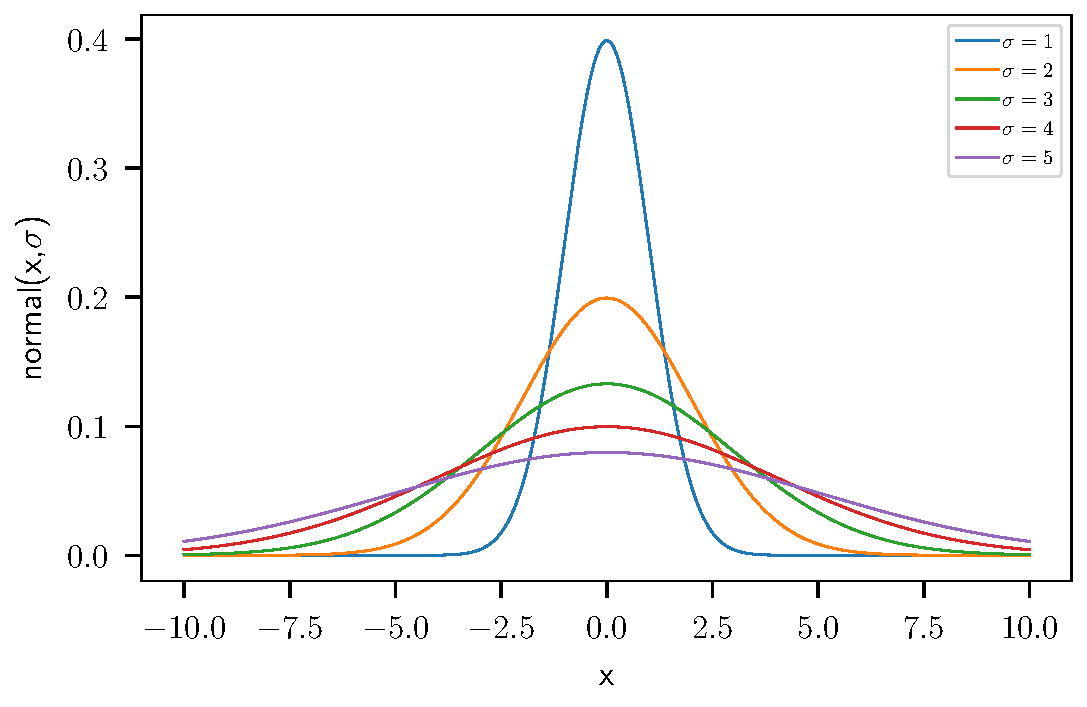
\includegraphics[width=15cm]{normal_dist}
	\caption{Plots of normal distributions for different values of $\sigma$. Larger $\sigma$ results in a broader distribution.}
	\label{fig}
\end{figure}

In order to satisfy equation (5), it must be true that $A=\frac{M}{\int_{x_i}^{x_f}e^{-\frac{1}{2}\left(\frac{x}{\sigma}\right)^2}dx}$, and therefore $\lambda(x)$ is given by:
\begin{equation}
	\lambda(x)=M\frac{e^{-\frac{1}{2}\left(\frac{x}{\sigma}\right)^2}}{\int_{x_i}^{x_f}e^{-\frac{1}{2}\left(\frac{x}{\sigma}\right)^2}dx}
\end{equation}
To calculate the moment of inertia, combine equation (7) with equation (4):
\begin{equation}
	I=\frac{M}{\int_{-\frac{L}{2}}^{\frac{L}{2}}e^{-\frac{1}{2}\left(\frac{x}{\sigma}\right)^2}dx}\int_{-\frac{L}{2}}^{\frac{L}{2}}x^2e^{-\frac{1}{2}\left(\frac{x}{\sigma}\right)^2}dx
\end{equation}
$M$ and $L$ will be global constants in your program (just set them both equal to 1); you will be estimating this integral for different values of $\sigma$. 

\subsection*{Uncertainty}
Note that you will be evaluating two separate integrals, each with an associated uncertainty which you will calculate as we did in class. The moment of inertia $I$ will therefore have its own associated uncertainty, which is a combination of the uncertainty of each integral. The uncertainties combine in the following way:

if $z_1=\int_{-\frac{L}{2}}^{\frac{L}{2}}x^2e^{-\frac{1}{2}\left(\frac{x}{\sigma}\right)^2}dx$, with uncertainty $\Delta z_1$, and $z_2=\int_{-\frac{L}{2}}^{\frac{L}{2}}e^{-\frac{1}{2}\left(\frac{x}{\sigma}\right)^2}dx$ with uncertainty $\Delta z_2$, then $I_{tot} = M\frac{z_1}{z_2}$, and $\Delta I_{tot}=M\left(\frac{\Delta z_1}{z_1}+\frac{\Delta z_2}{z_2}\right)I_{tot}$.

\subsection*{TL;DR}
You will write a program to calculate the moment of inertia of a thin rod whose mass is distributed as a normal distribution with standard deviation $\sigma$. The user will supply $\sigma$ and $n$ (the number of rectangles to use), and your program will print a Riemann estimate of $I$ together with the uncertainty on the estimate.
\subsection*{Requirements}
Your program should follow the style and readability guidelines detailed \href{https://drive.google.com/file/d/1SFf6Rhv8LydlrUhf85QhMuiZb_IKRS4N/view?usp=sharing}{here}
\end{document}